\chapter{Einleitung}

\section{Motivation}

\myboxy{
	\begin{itemize}
		\item ggf. auf die Röhre eingehen und die gesamte Technik erklären.
		\item Den Satz mit Elon Musk entfernen und die Geschichte von Hyperloop erklären.
	\end{itemize}
}{To-do}{\textwidth}


Der Hyperloop ist ein Konzept für ein Hochgeschwindigkeitstransportsystem, das von Elon Musk \cite{tesla:Hyperloop_impact} populär gemacht wurde. Es besteht im Wesentlichen aus einer oder mehreren Kapseln, die sich durch fast luftleere Röhren bewegen. Die Idee ist, Reibung und Luftwiderstand, die zwei größten Hindernisse für hohe Geschwindigkeiten, zu minimieren.

Durch die Reduzierung von Luft- und Rollwiderstand können Hyperloop-Kapseln Geschwindigkeiten von über 600 km/h erreichen. Dies ermöglicht extrem schnelle Reisen zwischen Städten, die weit voneinander entfernt sind.

Angesichts der globalen Bemühungen zur Reduzierung der CO2-Emissionen und zur Bekämpfung des Klimawandels könnte Hyperloop eine umweltfreundlichere Alternative zu Autos und Flugzeugen bieten.



\subsection{Institute of Hyperloop Technology}
Die Hochschule Emden/Leer hat im Jahr 2021 das Institut für Hyperloop-Technologie (IHT) gegründet, um aktiv an der Forschung zu dieser zukunftsweisenden Technologie teilzunehmen.

Im Rahmen dieser Forschung wurde an der Hochschule Emden eine Teststrecke mit einer Länge von 26 Metern errichtet (siehe Abbildung \ref{img_1_1:strecke}). Auf dieser Strecke soll das Fahrzeug (POD) unter realistischen Bedingungen getestet und weiterentwickelt werden.

\textbf{----------------------------------}\newline
Darüber hinaus engagiert sich das IHT in verschiedenen Projekten, darunter das \frqq European Hyperloop Technology Center – EuHyTeC\flqq, das europäische Hyperloop-Initiativen vernetzt und gemeinsam die nächste Generation des Transports entwickelt.\newline
\textbf{----------------------------------}

\begin{figure}[ht]
	\begin{center}
		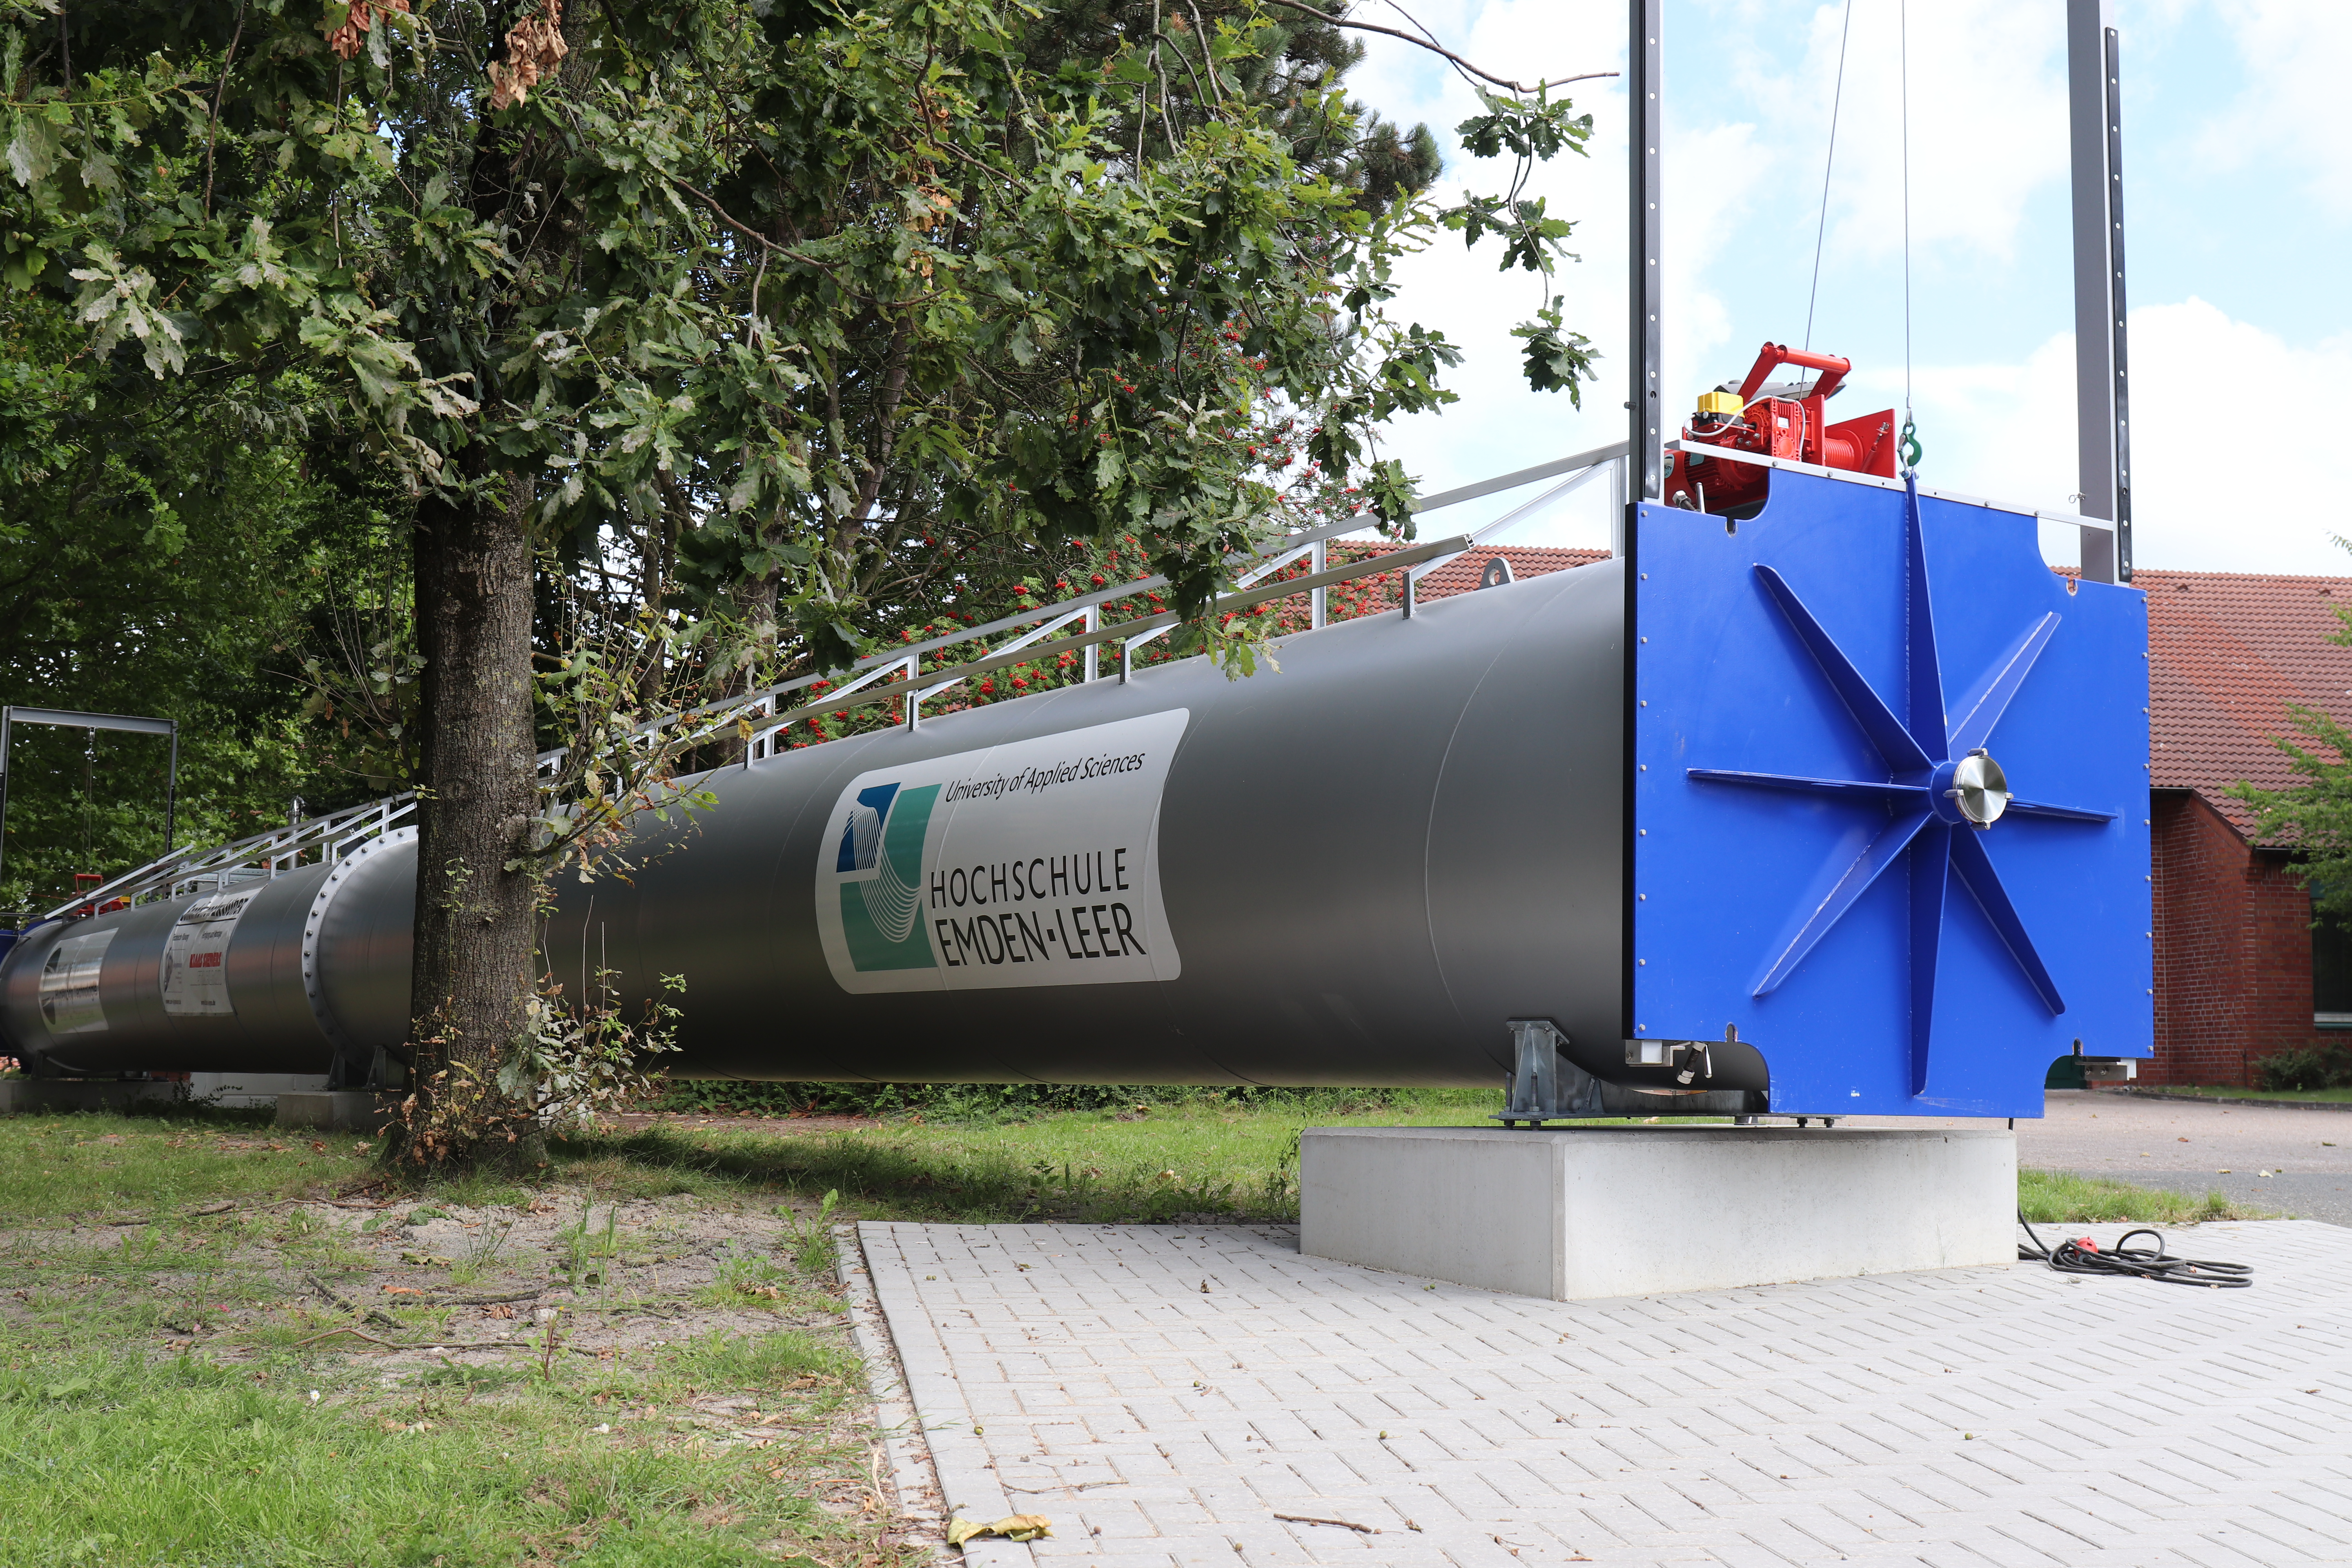
\includegraphics[width=\textwidth]{img/1_strecke/strecke_1.png}
		\caption{Hyperloop der Hochschule Emden Leer}
		\label{img_1_1:strecke}
	\end{center}
\end{figure}
\newpage

%Das neue Design des 48-Volt-Pods ist darauf ausgelegt, Material zu transportieren. Das Konzept sieht vor, dass eine große Lagerhalle am Stadtrand die Waren annimmt und sie dann durch das unterirdische Schienennetz zu den verschiedenen Standorten befördert. Auf diese Weise soll das Verkehrsaufkommen in den Städten durch Lastkraftwagen minimiert werden.


\section{Aufgabenstellung}
\myboxy{
	\begin{itemize}
		\item Ablauforientiert erklären. Also erst die Bestellung, dann der Schaltplan und dann die Simulation mit Simulink.
		\item Aufgabenstellung in der Vergangenheit formulieren.
		\item Den Leser in der Doku struktur Einführen. Am enden in 1.x
		\item Hinweis Test und Textergebnisse und in Betriebnahme entfallen.
	\end{itemize}
}{To-do}{\textwidth}


Die Motivation für dieses Projekt liegt in der Entwicklung eines Hyperloop-Fahrzeugs, das mit einer Batterie und einem Motor betrieben wird. Für die Steuerung des Fahrzeuges wurde ein echtzeitfähiges Steuerungsystem der Firma Speedgoat vorgeben, welches in Abschnitt \ref{sec:speedgoat} vertieft wird.\\ \ \\

Im Rahmen des Projekts wird ein Pod für den Hyperloop mit einer Bordspannung von 48 V konzipiert. Ziel ist es, die Machbarkeit dieser Spannung zu überprüfen und umzusetzen. Dazu gehören die Planung und Simulierung, die Integration der erforderlichen Sensorik sowie die Beschaffung der notwendigen Bauteile. Die Logik- und Signalverarbeitung wird mithilfe von Simulink auf dem echtzeitfähigen Speedgoat-System durchgeführt.
Die Steuerung erfolgt über Simulink, ein Modul von MATLAB, und umfasst die Erfassung von Position und Beschleunigung des Pods. Der Motor wird über ein zusätzliches Steuergerät angesteuert. Die Steuerung soll als Automatensteuerung umgesetzt werden.
Die Verdrahtung des Pods wird entsprechend der Bordspannung von 48 V ausgelegt. Hierfür wird mit der Software QElectroTech ein Schaltplan erstellt.
Alle erforderlichen Bauteile für die Umsetzung der Bordspannung, die Verdrahtung und die Sensorik müssen beschafft werden.

\textbf{----------------------------------}\newline
Entwurf und in Betriebnahme.
\textbf{----------------------------------}

\pagebreak

\section{Aufbau der Projektdokumentation }
